\documentclass{book}

\input{../activities-preamble.tex}
\begin{document}
\setcounter{cpjt}{64}
\addtocounter{cpjt}{-1}
\begin{activity}\label{act-latticepaths}
\hypertarget{p-483}{}%
The \terminology{integer lattice} is the set of all points in the Cartesian plane for which both the \(x\) and \(y\) coordinates are integers.%
\par
\hypertarget{p-484}{}%
A \terminology{lattice path}\index{lattice path} is one of the shortest possible paths connecting two points on the lattice, moving only horizontally and vertically. For example, here are three possible lattice paths from the points \((0,0)\) to \((3,2)\):%
\begin{sidebyside}{3}{0.0166666666666667}{0.0166666666666667}{0.0333333333333333}
\begin{sbspanel}{0.3}
\resizebox{\linewidth}{!}{{
      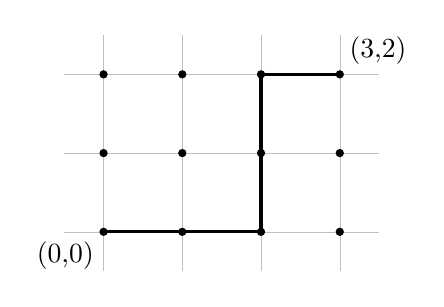
\begin{tikzpicture}
  \draw[very thin, color=gray!50] (-.5,-.5) grid (3.5, 2.5);
  \foreach \x in {0,...,3}
  \foreach \y in {0,...,2}
  \fill (\x,\y) circle (1.5pt);
  \draw (0,0) node[below left] { (0,0)} (3,2) node[above right] { (3,2)};
  \draw[very thick] (0,0) -- (2,0) -- (2,2) -- (3,2);
\end{tikzpicture}
}
}
\end{sbspanel}
\begin{sbspanel}{0.3}
\resizebox{\linewidth}{!}{{
      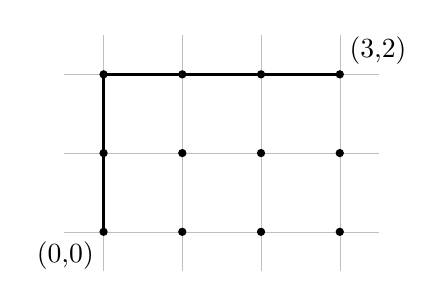
\begin{tikzpicture}
  \draw[very thin, color=gray!50] (-.5,-.5) grid (3.5, 2.5);
  \foreach \x in {0,...,3}
  \foreach \y in {0,...,2}
  \fill (\x,\y) circle (1.5pt);
  \draw (0,0) node[below left] { (0,0)} (3,2) node[above right] { (3,2)};
  \draw[very thick] (0,0) -- (0,2) -- (3,2);
\end{tikzpicture}
}
}
\end{sbspanel}
\begin{sbspanel}{0.3}
\resizebox{\linewidth}{!}{{
      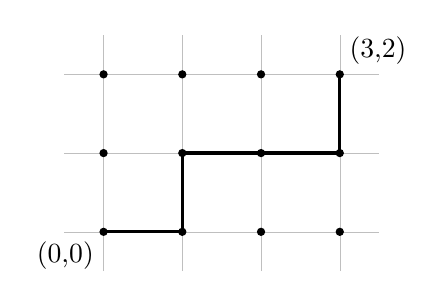
\begin{tikzpicture}
  \draw[very thin, color=gray!50] (-.5,-.5) grid (3.5, 2.5);
  \foreach \x in {0,...,3}
  \foreach \y in {0,...,2}
  \fill (\x,\y) circle (1.5pt);
  \draw (0,0) node[below left] { (0,0)} (3,2) node[above right] { (3,2)};
  \draw[very thick] (0,0) -- (1,0) -- (1,1) -- (3,1) -- (3,2);
\end{tikzpicture}
}
}
\end{sbspanel}
\end{sidebyside}
\begin{enumerate}[font=\bfseries,label=(\alph*),ref=\alph*]
\item\label{task-76} \hypertarget{p-485}{}%
How many lattice paths are there between \((0,0)\) and \((3,1)\)?  Draw or list them all (you might want to invent some notation for describing a path without drawing it).%
\item\label{task-77} \hypertarget{p-486}{}%
How many lattice paths are there between \((0,0)\) and \((2,2)\)? Draw or list them all to be sure.%
\item\label{task-78} \hypertarget{p-487}{}%
How many lattice paths are there between \((0,0)\) and \((3,2)\)? How can you be sure?%
\end{enumerate}
\end{activity}

\clearpage\end{document}
